% This article has been prepared for publication in Energy Economics in RStudio with knitr.
% According to http://www.elsevier.com/author-schemas/the-elsarticle-latex-document-class, we should be using the
% elsarticle.cls file.
% According to http://cdn.elsevier.com/assets/pdf_file/0006/109392/journal_refstyles.pdf, we should be using
% elsarticle-template-2-harv.tex as the template for the text.
% Furthermore, we should be using model2-names.bst for the bibliographic references.
% The approach here is to load the frontmatter and backmatter from elsarticle-template-2-harv.tex
% both ahead of and behind the text for our paper.
% -- Matthew Kuperus Heun, 2013-01-18

%% This is file `elsarticle-template-2-harv.tex',
%%
%% Copyright 2009 Elsevier Ltd
%%
%% This file is part of the 'Elsarticle  Bundle'.
%% ---------------------------------------------
%%
%% It may be distributed under the conditions of the LaTeX Project Public
%% License, either version 1.2 of this license or (at your option) any
%% later version.  The latest version of this license is in
%%    http://www.latex-project.org/lppl.txt
%% and version 1.2 or later is part of all distributions of LaTeX
%% version 1999/12/01 or later.
%%
%% The list of all files belonging to the 'Elsarticle Bundle' is
%% given in the file `manifest.txt'.
%%
%% Template article for Elsevier's document class `elsarticle'
%% with harvard style bibliographic references
%%
%% $Id: elsarticle-template-2-harv.tex 155 2009-10-08 05:35:05Z rishi $
%% $URL: http://lenova.river-valley.com/svn/elsbst/trunk/elsarticle-template-2-harv.tex $
%%
\documentclass[preprint,authoryear,12pt]{elsarticle}\usepackage{graphicx, color}
%% maxwidth is the original width if it is less than linewidth
%% otherwise use linewidth (to make sure the graphics do not exceed the margin)
\makeatletter
\def\maxwidth{ %
  \ifdim\Gin@nat@width>\linewidth
    \linewidth
  \else
    \Gin@nat@width
  \fi
}
\makeatother

\IfFileExists{upquote.sty}{\usepackage{upquote}}{}
\definecolor{fgcolor}{rgb}{0.2, 0.2, 0.2}
\newcommand{\hlnumber}[1]{\textcolor[rgb]{0,0,0}{#1}}%
\newcommand{\hlfunctioncall}[1]{\textcolor[rgb]{0.501960784313725,0,0.329411764705882}{\textbf{#1}}}%
\newcommand{\hlstring}[1]{\textcolor[rgb]{0.6,0.6,1}{#1}}%
\newcommand{\hlkeyword}[1]{\textcolor[rgb]{0,0,0}{\textbf{#1}}}%
\newcommand{\hlargument}[1]{\textcolor[rgb]{0.690196078431373,0.250980392156863,0.0196078431372549}{#1}}%
\newcommand{\hlcomment}[1]{\textcolor[rgb]{0.180392156862745,0.6,0.341176470588235}{#1}}%
\newcommand{\hlroxygencomment}[1]{\textcolor[rgb]{0.43921568627451,0.47843137254902,0.701960784313725}{#1}}%
\newcommand{\hlformalargs}[1]{\textcolor[rgb]{0.690196078431373,0.250980392156863,0.0196078431372549}{#1}}%
\newcommand{\hleqformalargs}[1]{\textcolor[rgb]{0.690196078431373,0.250980392156863,0.0196078431372549}{#1}}%
\newcommand{\hlassignement}[1]{\textcolor[rgb]{0,0,0}{\textbf{#1}}}%
\newcommand{\hlpackage}[1]{\textcolor[rgb]{0.588235294117647,0.709803921568627,0.145098039215686}{#1}}%
\newcommand{\hlslot}[1]{\textit{#1}}%
\newcommand{\hlsymbol}[1]{\textcolor[rgb]{0,0,0}{#1}}%
\newcommand{\hlprompt}[1]{\textcolor[rgb]{0.2,0.2,0.2}{#1}}%

\usepackage{framed}
\makeatletter
\newenvironment{kframe}{%
 \def\at@end@of@kframe{}%
 \ifinner\ifhmode%
  \def\at@end@of@kframe{\end{minipage}}%
  \begin{minipage}{\columnwidth}%
 \fi\fi%
 \def\FrameCommand##1{\hskip\@totalleftmargin \hskip-\fboxsep
 \colorbox{shadecolor}{##1}\hskip-\fboxsep
     % There is no \\@totalrightmargin, so:
     \hskip-\linewidth \hskip-\@totalleftmargin \hskip\columnwidth}%
 \MakeFramed {\advance\hsize-\width
   \@totalleftmargin\z@ \linewidth\hsize
   \@setminipage}}%
 {\par\unskip\endMakeFramed%
 \at@end@of@kframe}
\makeatother

\definecolor{shadecolor}{rgb}{.97, .97, .97}
\definecolor{messagecolor}{rgb}{0, 0, 0}
\definecolor{warningcolor}{rgb}{1, 0, 1}
\definecolor{errorcolor}{rgb}{1, 0, 0}
\newenvironment{knitrout}{}{} % an empty environment to be redefined in TeX

\usepackage{alltt}

%% Use the option review to obtain double line spacing
%% \documentclass[authoryear,preprint,review,12pt]{elsarticle}

%% Use the options 1p,twocolumn; 3p; 3p,twocolumn; 5p; or 5p,twocolumn
%% for a journal layout:
%% \documentclass[final,authoryear,1p,times]{elsarticle}
%% \documentclass[final,authoryear,1p,times,twocolumn]{elsarticle}
%% \documentclass[final,authoryear,3p,times]{elsarticle}
%% \documentclass[final,authoryear,3p,times,twocolumn]{elsarticle}
%% \documentclass[final,authoryear,5p,times]{elsarticle}
%% \documentclass[final,authoryear,5p,times,twocolumn]{elsarticle}

%% if you use PostScript figures in your article
%% use the graphics package for simple commands
%% \usepackage{graphics}
%% or use the graphicx package for more complicated commands
%% \usepackage{graphicx}
%% or use the epsfig package if you prefer to use the old commands
%% \usepackage{epsfig}

%% The amssymb package provides various useful mathematical symbols
\usepackage{amssymb}
%% The amsthm package provides extended theorem environments
%% \usepackage{amsthm}

%% The lineno packages adds line numbers. Start line numbering with
%% \begin{linenumbers}, end it with \end{linenumbers}. Or switch it on
%% for the whole article with \linenumbers after \end{frontmatter}.
%% \usepackage{lineno}

%% natbib.sty is loaded by default. However, natbib options can be
%% provided with \biboptions{...} command. Following options are
%% valid:

%%   round  -  round parentheses are used (default)
%%   square -  square brackets are used   [option]
%%   curly  -  curly braces are used      {option}
%%   angle  -  angle brackets are used    <option>
%%   semicolon  -  multiple citations separated by semi-colon (default)
%%   colon  - same as semicolon, an earlier confusion
%%   comma  -  separated by comma
%%   authoryear - selects author-year citations (default)
%%   numbers-  selects numerical citations
%%   super  -  numerical citations as superscripts
%%   sort   -  sorts multiple citations according to order in ref. list
%%   sort&compress   -  like sort, but also compresses numerical citations
%%   compress - compresses without sorting
%%   longnamesfirst  -  makes first citation full author list
%%
%% \biboptions{longnamesfirst,comma}

% \biboptions{}

\journal{Energy Economics}

\begin{document}

\begin{frontmatter}

%% Title, authors and addresses

%% use the tnoteref command within \title for footnotes;
%% use the tnotetext command for the associated footnote;
%% use the fnref command within \author or \address for footnotes;
%% use the fntext command for the associated footnote;
%% use the corref command within \author for corresponding author footnotes;
%% use the cortext command for the associated footnote;
%% use the ead command for the email address,
%% and the form \ead[url] for the home page:
%%
%% \title{Title\tnoteref{label1}}
%% \tnotetext[label1]{}
%% \author{Name\corref{cor1}\fnref{label2}}
%% \ead{email address}
%% \ead[url]{home page}
%% \fntext[label2]{}
%% \cortext[cor1]{}
%% \address{Address\fnref{label3}}
%% \fntext[label3]{}

\title{Empirical Analysis of the Role of Energy in Economic Growth}

%% use optional labels to link authors explicitly to addresses:
%% \author[label1,label2]{<author name>}
%% \address[label1]{<address>}
%% \address[label2]{<address>}

\author[Calvin]{Caleb Reese}
\author[Calvin]{Lucas Timmer}
\author[Calvin]{Matthew Kuperus Heun \corref{cor1}}
\ead{mkh2@calvin.edu, tel: +1 (616) 526-6663, fax: +1 (616) 526-6501}

\cortext[cor1]{Corresponding author}
\address[Calvin]{Engineering Department, Calvin College, Grand Rapids, MI 49546, USA}

\begin{abstract}
%% Text of abstract
*********** Add abstract ***********
\end{abstract}

\begin{keyword}
%% keywords here, in the form: keyword \sep keyword
economic growth \sep energy \sep cobb-douglas \sep CES \sep LINEX
%% MSC codes here, in the form: \MSC code \sep code
%% or \MSC[2008] code \sep code (2000 is the default)
\end{keyword}

\end{frontmatter}

% \linenumbers
%% main text

Caleb, put your LaTeX code here.









\begin{knitrout}
\definecolor{shadecolor}{rgb}{0.969, 0.969, 0.969}\color{fgcolor}\begin{kframe}
\begin{alltt}
createCountryFactorsGraph <- \hlfunctioncall{function}(countryName)\{
  dataTable <- \hlfunctioncall{loadData}(countryName)
  graphType <- \hlstring{"l"}
  lineTypes <- \hlfunctioncall{c}(1, 5, 2, 4, 6) \hlcomment{#line types. See http://en.wikibooks.org/wiki/R_Programming/Graphics}
  lineWidths <- \hlfunctioncall{c}(1, 1, 1, 1, 1) \hlcomment{#line widths}
  colors <- \hlfunctioncall{c}(\hlstring{"black"}, \hlstring{"black"}, \hlstring{"black"}, \hlstring{"black"}, \hlstring{"black"}) #line and point colors
  lineSpec <- \hlfunctioncall{list}(lty=lineTypes, lwd=lineWidths, col=colors)
  graph <- \hlfunctioncall{xyplot}(iCapStk+iLabor+iQ+iX+iU ~ Year, data=dataTable,
                  type=graphType,
                  par.settings = \hlfunctioncall{list}(superpose.line = lineSpec),
                  key=\hlfunctioncall{list}(text=\hlfunctioncall{list}(\hlfunctioncall{c}(\hlstring{"k"}, \hlstring{"l"}, \hlstring{"q"}, \hlstring{"x"}, \hlstring{"u"})),
                           type=graphType,
                           lines=lineSpec,
                           columns=1, x=0.0, y=0.98),
                  scales=\hlfunctioncall{list}(cex=1.0, \hlcomment{#controls text size on scales}
                              tck=-0.5), \hlcomment{#controls tick mark length}
                  ylab=\hlstring{"\hlfunctioncall{Indexed} (1980=1)"})
  \hlfunctioncall{return}(graph)
\}

createFactorsLatticeGraph <- \hlfunctioncall{function}(countryName)\{
  dataTable <- \hlfunctioncall{loadData}(countryName)
  graphType <- \hlstring{"l"}
  lineTypes <- \hlfunctioncall{c}(1, 5, 2, 4, 6) \hlcomment{#line types. See http://en.wikibooks.org/wiki/R_Programming/Graphics}
  lineWidths <- \hlfunctioncall{c}(1, 1, 1, 1, 1) \hlcomment{#line widths}
  colors <- \hlfunctioncall{c}(\hlstring{"black"}, \hlstring{"black"}, \hlstring{"black"}, \hlstring{"black"}, \hlstring{"black"}) #line and point colors
  lineSpec <- \hlfunctioncall{list}(lty=lineTypes, lwd=lineWidths, col=colors)
  graph <- \hlfunctioncall{xyplot}(iCapStk+iLabor+iQ+iX+iU ~ Year | Country, data=dataTable,
                  type=graphType,
                  par.settings = \hlfunctioncall{list}(superpose.line = lineSpec),
                  key=\hlfunctioncall{list}(text=\hlfunctioncall{list}(\hlfunctioncall{c}(\hlstring{"k"}, \hlstring{"l"}, \hlstring{"q"}, \hlstring{"x"}, \hlstring{"u"})),
                           type=graphType,
                           cex=0.85,
                           lines=lineSpec,
                           columns=1, x=0.01, y=0.92),
                  scales=\hlfunctioncall{list}(cex=0.75, \hlcomment{#controls text size on scales}
                              tck=-0.5), \hlcomment{#controls tick mark length}
                  ylab=\hlstring{"\hlfunctioncall{Indexed} (1980=1)"})
  \hlfunctioncall{return}(graph)
\}

createGDPComparisonGraph <- \hlfunctioncall{function}(countryName)\{
  dataTable <- \hlfunctioncall{loadData}(countryName)
  graphType <- \hlstring{"l"}
  lineTypes <- \hlfunctioncall{c}(1) \hlcomment{#line types. See http://en.wikibooks.org/wiki/R_Programming/Graphics}
  lineWidths <- \hlfunctioncall{c}(1) \hlcomment{#line widths}
  colors <- \hlfunctioncall{c}(\hlstring{"black"}) #line and point colors
  lineSpec <- \hlfunctioncall{list}(lty=lineTypes, lwd=lineWidths, col=colors)
  graph <- \hlfunctioncall{xyplot}(iGDP ~ Year, data=dataTable,
                  key=\hlfunctioncall{list}(text=\hlfunctioncall{list}(\hlfunctioncall{c}(\hlstring{"GDP"})),
                           type=graphType,
                           lines=lineSpec,
                           columns=1, x=0.0, y=0.98),
                  type=graphType,
                  par.settings = \hlfunctioncall{list}(superpose.line = lineSpec),
                  scales=\hlfunctioncall{list}(cex=1.0, \hlcomment{#controls text size on scales}
                              tck=-0.5), \hlcomment{#controls tick mark length}
                  ylab=\hlstring{"\hlfunctioncall{Indexed} (1980=1)"})
  \hlfunctioncall{return}(graph)
\}


\hlcomment{# createGDPComparisonGraph <- function(countryName)\{}
\hlcomment{#   dataTable <- loadData(countryName)}
\hlcomment{#   graphType <- "l"}
\hlcomment{#   colors <- c("black", "black", "black", "black") #line and point colors}
\hlcomment{#   lineWidths <- c(1, 1, 1, 1) #line widths}
\hlcomment{#   lineTypes <- c(1, 5, 2, 4) #line types. See http://en.wikibooks.org/wiki/R_Programming/Graphics}
\hlcomment{#   lineSpec <- list(lty=lineTypes, lwd=lineWidths, col=colors)}
\hlcomment{#   pointSpec <- list(col=colors)}
\hlcomment{#   graph <- xyplot(iGDP ~ iYear, data=dataTable,}
\hlcomment{#                   key=list(text=list(c("GDP")),}
\hlcomment{#                            type=graphType,}
\hlcomment{#                            lines=lineSpec,}
\hlcomment{#                            columns=1, x=0.0, y=0.98),}
\hlcomment{#                   type=graphType,}
\hlcomment{#                   par.settings = list(superpose.line = lineSpec),}
\hlcomment{# #                                      superpose.symbol = pointSpec),}
\hlcomment{#                   scales=list(cex=1.0, #controls text size on scales}
\hlcomment{#                               tck=-0.5), #controls tick mark length}
\hlcomment{#                   ylab="Indexed (1980=1)")}
\hlcomment{#   return(graph)}
\hlcomment{# }
\hlcomment{#                     }
\hlcomment{# \}}


\hlfunctioncall{createFactorsLatticeGraph}(\hlstring{"All"})
\end{alltt}
\end{kframe}
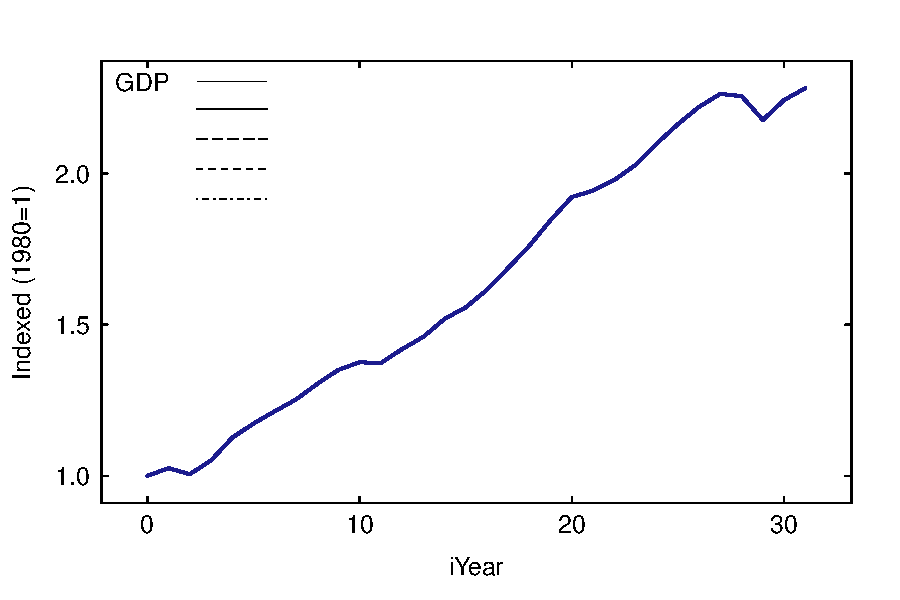
\includegraphics[width=\maxwidth]{figure/graphs} 
\begin{kframe}\begin{alltt}

\hlcomment{#createGDPComparisonGraph("US")}

\hlcomment{#createCountryFactorsGraph("US")}
\hlcomment{#lapply(countries, createCountryFactorsGraph)}



\end{alltt}
\end{kframe}
\end{knitrout}


\section{Cobb-Douglas Without Energy}

\begin{knitrout}
\definecolor{shadecolor}{rgb}{0.969, 0.969, 0.969}\color{fgcolor}\begin{kframe}
\begin{alltt}

\hlcomment{#################################################}
\hlcomment{# Calculates parameter estimates and confidence intervals}
\hlcomment{# for the Cobb-Douglas production function given a country.}
\hlcomment{#}
\hlcomment{# countryName is a string containing the 2-letter abbreviation for the country, e.g. "US" or "CN"}
\hlcomment{#}
\hlcomment{# returns a vector of data for the Cobb-Douglas model. }
\hlcomment{# First item is the +95% CI on all parameters}
\hlcomment{# Second item contains the parameter estimates}
\hlcomment{# Third item is the -95% CI on all parameters}
\hlcomment{# Each row has names: lambda, alpha, beta, gamma, corresponding to the parameters in the model.}
\hlcomment{##}
cobbDouglasData <- \hlfunctioncall{function}(countryName)\{
  
\hlcomment{  # Load the data that we need.}
  dataTable <- \hlfunctioncall{loadData}(countryName)
  
\hlcomment{  # Establish guess values for alpha and lambda.}
  lambdaGuess <- 0.0 \hlcomment{# guessing lambda = 0 means there is no technological progress.}
  alphaGuess <- 0.3 \hlcomment{# a typical value for alpha, the coefficient on capital stock}
  
\hlcomment{  # Runs a non-linear least squares fit to the data. We've replaced beta with 1-alpha for simplicity.}
  modelCD <- \hlfunctioncall{nls}(iGDP ~ \hlfunctioncall{exp}(lambda*iYear) * iCapStk^alpha * iLabor^(1 - alpha), 
\hlcomment{#                 algorithm = "port",}
                 start = \hlfunctioncall{list}(lambda=lambdaGuess, alpha=alphaGuess),
\hlcomment{#                 lower = list(lambda=-Inf, alpha=0),}
\hlcomment{#                 upper = list(lambda=Inf, alpha=1),}
                 data=dataTable)
  
\hlcomment{  # Checks validity of the model. AIC stands for Akaike's Information Criterion.}
  aicCD  <- \hlfunctioncall{AIC}(modelCD, k=2)
\hlcomment{  #print(aicCD)}
  
  summaryCD <- \hlfunctioncall{summary}(modelCD) \hlcomment{# Gives the nls summary table.}
\hlcomment{  #print(summaryCD)}
  ciCD <- \hlfunctioncall{confint}(modelCD, level = ciLevel); ciCD \hlcomment{# Displays confidence intervals for the CD model.}
  
\hlcomment{  # Calculate beta and its confidence interval and report it.}
  alpha <- \hlfunctioncall{as.numeric}(\hlfunctioncall{coef}(modelCD)[\hlstring{"alpha"}])
  beta <- 1.0 - alpha
  beta.est <- \hlfunctioncall{deltaMethod}(modelCD, \hlstring{"1 - alpha"}); beta.est # Estimates beta and its standard \hlfunctioncall{error} (SE).
\hlcomment{  # Now calculate a confidence interval on beta}
  dofCD <- summaryCD$df[2]; dofCD \hlcomment{# Gives the degrees of freedom for the model.}
  tvalCD <- \hlfunctioncall{qt}(ciHalfLevel, df = dofCD); tvalCD
  betaCICD <- \hlfunctioncall{with}(beta.est, Estimate + \hlfunctioncall{c}(-1.0, 1.0) * tvalCD * SE); betaCICD \hlcomment{# Gives the confidence interval on beta.}
  
\hlcomment{  #print(coef(modelCD))}
  
\hlcomment{  # Combine all estimates and their confidence intervals into data frames with intelligent row names}
  estCD <- \hlfunctioncall{data.frame}(lambda = \hlfunctioncall{coef}(modelCD)[\hlstring{"lambda"}], alpha = \hlfunctioncall{coef}(modelCD)[\hlstring{"alpha"}], beta = beta, gamma = 0)
\hlcomment{  #print(estCD)}
  \hlfunctioncall{row.names}(estCD) <- \hlstring{"CD"}
\hlcomment{  #row.names(estCD) <- "Cobb-Douglas: $y = e^\{\textbackslash{}\textbackslash{}lambda t\}k^\{\textbackslash{}\textbackslash{}alpha\}l^\{\textbackslash{}\textbackslash{}beta\}$"}
\hlcomment{  # The [1] subscripts pick off the lower confidence interval}
  lowerCD <- \hlfunctioncall{data.frame}(lambda = ciCD[\hlstring{"lambda"},\hlstring{"2.5%"}], alpha = ciCD[\hlstring{"alpha"}, \hlstring{"2.5%"}], beta = betaCICD[1], gamma = NA) 
  \hlfunctioncall{row.names}(lowerCD) <- \hlstring{"- 95% CI"}
\hlcomment{  # The [2] subscripts pick off the lower confidence interval}
  upperCD <- \hlfunctioncall{data.frame}(lambda = ciCD[\hlstring{"lambda"},\hlstring{"97.5%"}], alpha = ciCD[\hlstring{"alpha"}, \hlstring{"97.5%"}], beta = betaCICD[2], gamma = NA)
  \hlfunctioncall{row.names}(upperCD) <- \hlstring{"+ 95% CI"}
  
\hlcomment{  # Now create the data for a table.}
  dataCD <- \hlfunctioncall{rbind}(upperCD, estCD, lowerCD)
\hlcomment{  #print(dataCD)}
  \hlfunctioncall{return}(dataCD)
\}

\hlcomment{####################################}
\hlcomment{# Creates a LaTeX printable table from the Cobb Douglas data. This function first calls cobbDouglasData.}
\hlcomment{#}
\hlcomment{# countryName is a string containint the 2-letter abbreviation for the country, e.g. "US" or "CN"}
\hlcomment{#}
\hlcomment{# returns a printable LaTeX table from xtable.}
\hlcomment{##}
cobbDouglasTable <- \hlfunctioncall{function}(countryName)\{
  dataCD <- \hlfunctioncall{cobbDouglasData}(countryName) 
  \hlfunctioncall{colnames}(dataCD) <- \hlfunctioncall{c}(\hlstring{"$\textbackslash{}\textbackslash{}lambda$"}, \hlstring{"$\textbackslash{}\textbackslash{}alpha$"}, \hlstring{"$\textbackslash{}\textbackslash{}beta$"}, \hlstring{"$\textbackslash{}\textbackslash{}gamma$"})
  tableCD <- \hlfunctioncall{xtable}(dataCD, caption=\hlfunctioncall{paste}(countryName, \hlstring{" Cobb-Douglas, 1980-2011"}, sep=\hlstring{""}), digit = \hlfunctioncall{c}(4, 4, 2, 2, 1))
\hlcomment{  #print(tableCD)}
  \hlfunctioncall{return}(tableCD)  
\}
\end{alltt}
\end{kframe}
\end{knitrout}


\begin{knitrout}
\definecolor{shadecolor}{rgb}{0.969, 0.969, 0.969}\color{fgcolor}\begin{kframe}
\begin{alltt}
tablesCD <- \hlfunctioncall{lapply}(countries, cobbDouglasTable)
\end{alltt}


{\ttfamily\noindent\itshape\color{messagecolor}{Waiting for profiling to be done...}}

{\ttfamily\noindent\itshape\color{messagecolor}{Waiting for profiling to be done...}}

{\ttfamily\noindent\itshape\color{messagecolor}{Waiting for profiling to be done...}}

{\ttfamily\noindent\itshape\color{messagecolor}{Waiting for profiling to be done...}}

{\ttfamily\noindent\itshape\color{messagecolor}{Waiting for profiling to be done...}}

{\ttfamily\noindent\itshape\color{messagecolor}{Waiting for profiling to be done...}}

{\ttfamily\noindent\itshape\color{messagecolor}{Waiting for profiling to be done...}}

{\ttfamily\noindent\itshape\color{messagecolor}{Waiting for profiling to be done...}}

{\ttfamily\noindent\itshape\color{messagecolor}{Waiting for profiling to be done...}}\end{kframe}
\end{knitrout}


\begin{kframe}
\begin{alltt}
\hlfunctioncall{print}(tablesCD[[\hlstring{"US"}]], caption.placement=\hlstring{"top"})
\end{alltt}
\end{kframe}% latex table generated in R 2.15.2 by xtable 1.7-0 package
% Sun Jan 27 13:40:21 2013
\begin{table}[ht]
\begin{center}
\caption{US Cobb-Douglas, 1980-2011}
\begin{tabular}{rrrrr}
  \hline
 & \$$\backslash$lambda\$ & \$$\backslash$alpha\$ & \$$\backslash$beta\$ & \$$\backslash$gamma\$ \\ 
  \hline
+ 95\% CI & 0.0116 & 0.34 & 0.79 &  \\ 
  CD & 0.0102 & 0.27 & 0.73 & 0.0 \\ 
  - 95\% CI & 0.0087 & 0.21 & 0.66 &  \\ 
   \hline
\end{tabular}
\end{center}
\end{table}
\begin{kframe}\begin{alltt}
\hlfunctioncall{print}(tablesCD[[\hlstring{"UK"}]], caption.placement=\hlstring{"top"})
\end{alltt}
\end{kframe}% latex table generated in R 2.15.2 by xtable 1.7-0 package
% Sun Jan 27 13:40:21 2013
\begin{table}[ht]
\begin{center}
\caption{UK Cobb-Douglas, 1980-2011}
\begin{tabular}{rrrrr}
  \hline
 & \$$\backslash$lambda\$ & \$$\backslash$alpha\$ & \$$\backslash$beta\$ & \$$\backslash$gamma\$ \\ 
  \hline
+ 95\% CI & 0.0303 & 1.12 & 1.24 &  \\ 
  CD & 0.0097 & 0.44 & 0.56 & 0.0 \\ 
  - 95\% CI & -0.0104 & -0.25 & -0.13 &  \\ 
   \hline
\end{tabular}
\end{center}
\end{table}
\begin{kframe}\begin{alltt}
\hlfunctioncall{print}(tablesCD[[\hlstring{"JP"}]], caption.placement=\hlstring{"top"})
\end{alltt}
\end{kframe}% latex table generated in R 2.15.2 by xtable 1.7-0 package
% Sun Jan 27 13:40:21 2013
\begin{table}[ht]
\begin{center}
\caption{JP Cobb-Douglas, 1980-2011}
\begin{tabular}{rrrrr}
  \hline
 & \$$\backslash$lambda\$ & \$$\backslash$alpha\$ & \$$\backslash$beta\$ & \$$\backslash$gamma\$ \\ 
  \hline
+ 95\% CI & 0.0081 & 0.61 & 0.56 &  \\ 
  CD & 0.0048 & 0.52 & 0.48 & 0.0 \\ 
  - 95\% CI & 0.0014 & 0.44 & 0.39 &  \\ 
   \hline
\end{tabular}
\end{center}
\end{table}
\begin{kframe}\begin{alltt}
\hlfunctioncall{print}(tablesCD[[\hlstring{"ZA"}]], caption.placement=\hlstring{"top"})
\end{alltt}
\end{kframe}% latex table generated in R 2.15.2 by xtable 1.7-0 package
% Sun Jan 27 13:40:21 2013
\begin{table}[ht]
\begin{center}
\caption{ZA Cobb-Douglas, 1980-2011}
\begin{tabular}{rrrrr}
  \hline
 & \$$\backslash$lambda\$ & \$$\backslash$alpha\$ & \$$\backslash$beta\$ & \$$\backslash$gamma\$ \\ 
  \hline
+ 95\% CI & 0.0022 & 0.73 & 0.54 &  \\ 
  CD & 0.0008 & 0.60 & 0.40 & 0.0 \\ 
  - 95\% CI & -0.0007 & 0.46 & 0.26 &  \\ 
   \hline
\end{tabular}
\end{center}
\end{table}
\begin{kframe}\begin{alltt}
\hlfunctioncall{print}(tablesCD[[\hlstring{"CN"}]], caption.placement=\hlstring{"top"})
\end{alltt}
\end{kframe}% latex table generated in R 2.15.2 by xtable 1.7-0 package
% Sun Jan 27 13:40:21 2013
\begin{table}[ht]
\begin{center}
\caption{CN Cobb-Douglas, 1980-2011}
\begin{tabular}{rrrrr}
  \hline
 & \$$\backslash$lambda\$ & \$$\backslash$alpha\$ & \$$\backslash$beta\$ & \$$\backslash$gamma\$ \\ 
  \hline
+ 95\% CI & 0.0779 & 1.32 & 0.89 &  \\ 
  CD & 0.0188 & 0.71 & 0.29 & 0.0 \\ 
  - 95\% CI & -0.0405 & 0.11 & -0.32 &  \\ 
   \hline
\end{tabular}
\end{center}
\end{table}
\begin{kframe}\begin{alltt}
\hlfunctioncall{print}(tablesCD[[\hlstring{"SA"}]], caption.placement=\hlstring{"top"})
\end{alltt}
\end{kframe}% latex table generated in R 2.15.2 by xtable 1.7-0 package
% Sun Jan 27 13:40:21 2013
\begin{table}[ht]
\begin{center}
\caption{SA Cobb-Douglas, 1980-2011}
\begin{tabular}{rrrrr}
  \hline
 & \$$\backslash$lambda\$ & \$$\backslash$alpha\$ & \$$\backslash$beta\$ & \$$\backslash$gamma\$ \\ 
  \hline
+ 95\% CI & -0.0087 & 0.68 & 0.78 &  \\ 
  CD & -0.0123 & 0.45 & 0.55 & 0.0 \\ 
  - 95\% CI & -0.0159 & 0.21 & 0.32 &  \\ 
   \hline
\end{tabular}
\end{center}
\end{table}
\begin{kframe}\begin{alltt}
\hlfunctioncall{print}(tablesCD[[\hlstring{"IR"}]], caption.placement=\hlstring{"top"})
\end{alltt}
\end{kframe}% latex table generated in R 2.15.2 by xtable 1.7-0 package
% Sun Jan 27 13:40:21 2013
\begin{table}[ht]
\begin{center}
\caption{IR Cobb-Douglas, 1980-2011}
\begin{tabular}{rrrrr}
  \hline
 & \$$\backslash$lambda\$ & \$$\backslash$alpha\$ & \$$\backslash$beta\$ & \$$\backslash$gamma\$ \\ 
  \hline
+ 95\% CI & 0.0045 & 0.70 & 0.51 &  \\ 
  CD & 0.0039 & 0.60 & 0.40 & 0.0 \\ 
  - 95\% CI & 0.0032 & 0.49 & 0.30 &  \\ 
   \hline
\end{tabular}
\end{center}
\end{table}
\begin{kframe}\begin{alltt}
\hlfunctioncall{print}(tablesCD[[\hlstring{"TZ"}]], caption.placement=\hlstring{"top"})
\end{alltt}
\end{kframe}% latex table generated in R 2.15.2 by xtable 1.7-0 package
% Sun Jan 27 13:40:21 2013
\begin{table}[ht]
\begin{center}
\caption{TZ Cobb-Douglas, 1980-2011}
\begin{tabular}{rrrrr}
  \hline
 & \$$\backslash$lambda\$ & \$$\backslash$alpha\$ & \$$\backslash$beta\$ & \$$\backslash$gamma\$ \\ 
  \hline
+ 95\% CI & 0.0068 & 0.95 & 0.50 &  \\ 
  CD & 0.0015 & 0.73 & 0.27 & 0.0 \\ 
  - 95\% CI & -0.0039 & 0.50 & 0.05 &  \\ 
   \hline
\end{tabular}
\end{center}
\end{table}
\begin{kframe}\begin{alltt}
\hlfunctioncall{print}(tablesCD[[\hlstring{"ZM"}]], caption.placement=\hlstring{"top"})
\end{alltt}
\end{kframe}% latex table generated in R 2.15.2 by xtable 1.7-0 package
% Sun Jan 27 13:40:21 2013
\begin{table}[ht]
\begin{center}
\caption{ZM Cobb-Douglas, 1980-2011}
\begin{tabular}{rrrrr}
  \hline
 & \$$\backslash$lambda\$ & \$$\backslash$alpha\$ & \$$\backslash$beta\$ & \$$\backslash$gamma\$ \\ 
  \hline
+ 95\% CI & 0.0280 & 1.57 & -0.25 &  \\ 
  CD & 0.0249 & 1.41 & -0.41 & 0.0 \\ 
  - 95\% CI & 0.0218 & 1.25 & -0.57 &  \\ 
   \hline
\end{tabular}
\end{center}
\end{table}
\begin{kframe}\begin{alltt}

\hlcomment{# According to http://cran.r-project.org/web/packages/xtable/vignettes/xtableGallery.pdf, Section 3.1, I should }
\hlcomment{# be able to use the "sanitize.text.function" parameter to allow markup in column headers. But this next}
\hlcomment{# line is not working at the present time. --MKH, 18 Jan 2012.}
\hlcomment{# print(tableCD, caption.placement="top", sanitize.text.function = function(x)\{x\})}
\end{alltt}
\end{kframe}


\section{Cobb-Douglas With Energy}

We can force $\alpha$, $\beta$, and $\gamma$ to be in $[0,1]$ by a reparameterization:

\[ a \in[0,1], b \in [0,1], \alpha=\min(a,b), \beta=|b-a|, \gamma = 1-\max(a,b) \]




\subsection{Cobb-Douglas with $Q$}

\begin{knitrout}
\definecolor{shadecolor}{rgb}{0.969, 0.969, 0.969}\color{fgcolor}\begin{kframe}
\begin{alltt}
\hlcomment{# Note that the anlaysis of ZA is taking a long time here. Need to figure out why.}
CDqTables <- \hlfunctioncall{lapply}(countries, cobbDouglasEnergyTable, energyType=\hlstring{"Q"})
\end{alltt}
\end{kframe}
\end{knitrout}


\begin{kframe}
\begin{alltt}
\hlfunctioncall{print}(CDqTables[[\hlstring{"US"}]], caption.placement=\hlstring{"top"})
\hlfunctioncall{print}(CDqTables[[\hlstring{"ZA"}]], caption.placement=\hlstring{"top"})
\hlcomment{# According to http://cran.r-project.org/web/packages/xtable/vignettes/xtableGallery.pdf, Section 3.1, I should }
\hlcomment{# be able to use the "sanitize.text.function" parameter to allow markup in column headers. But this next}
\hlcomment{# line is not working at the present time. --MKH, 18 Jan 2012.}
\hlcomment{# print(tableCDe, sanitize.text.function = function(x)\{x\})}

\hlcomment{#print(tableAll, caption.placement="top")}
\end{alltt}
\end{kframe}


\subsection{Cobb-Douglas With $X$}

\begin{knitrout}
\definecolor{shadecolor}{rgb}{0.969, 0.969, 0.969}\color{fgcolor}\begin{kframe}
\begin{alltt}
\hlcomment{# Note that the anlaysis of ZA is taking a long time here. Need to figure out why.}
CDxTables <- \hlfunctioncall{lapply}(countries, cobbDouglasEnergyTable, energyType=\hlstring{"X"})
\end{alltt}
\end{kframe}
\end{knitrout}


\begin{kframe}
\begin{alltt}
\hlfunctioncall{print}(CDxTables[[\hlstring{"US"}]], caption.placement=\hlstring{"top"})
\hlfunctioncall{print}(CDxTables[[\hlstring{"ZA"}]], caption.placement=\hlstring{"top"})
\end{alltt}
\end{kframe}


\subsection{Cobb-Douglas With $U$}

\begin{knitrout}
\definecolor{shadecolor}{rgb}{0.969, 0.969, 0.969}\color{fgcolor}\begin{kframe}
\begin{alltt}
CDuTables <- \hlfunctioncall{lapply}(countries, cobbDouglasEnergyTable, energyType=\hlstring{"U"})
\end{alltt}
\end{kframe}
\end{knitrout}


\begin{kframe}
\begin{alltt}
\hlfunctioncall{print}(CDuTables[[\hlstring{"US"}]], caption.placement=\hlstring{"top"})
\hlfunctioncall{print}(CDuTables[[\hlstring{"ZA"}]], caption.placement=\hlstring{"top"})
\end{alltt}
\end{kframe}


\section{CES}

\begin{knitrout}
\definecolor{shadecolor}{rgb}{0.969, 0.969, 0.969}\color{fgcolor}\begin{kframe}
\begin{alltt}
cesData <- \hlfunctioncall{function}(countryName, energyType)\{
  energyColumnName <- \hlfunctioncall{paste}(\hlstring{"i"}, energyType, sep=\hlstring{""})
\hlcomment{  # Load the data that we need.}
  dataTable <- \hlfunctioncall{loadData}(countryName)
    
\hlcomment{  # Establish guess values for phi beta, zeta, lambda_L and lambda_E.}
  phiGuess <- -20
  betaGuess <- 0.5 \hlcomment{# a typical value for \hlfunctioncall{beta} (exponent on labor)}
  zetaGuess <- 0.0004 \hlcomment{# a small value}
  lambda_LGuess <- 0.007 \hlcomment{#assuming no technical progress on the labor-capital portion of the function}
  lambda_EGuess <- 0.008 \hlcomment{#assuming no technical progress on the energy portion of the function}
  
\hlcomment{  # Runs a non-linear least squares fit to the data with constraints}
  modelCES <- \hlfunctioncall{nls}(iGDP ~ ((1-zeta) * (\hlfunctioncall{exp}(lambda_L*iYear) * iCapStk^(1-beta) * iLabor^beta)^phi 
                           + zeta*(\hlfunctioncall{exp}(lambda_E*iYear) * iQ)^phi)^(1/phi), 
                   algorithm = \hlstring{"port"},
                   control = \hlfunctioncall{nls.control}(maxiter = 500, tol = 1e-06, minFactor = 1/1024, 
                                         printEval = FALSE, warnOnly = FALSE),
                   start = \hlfunctioncall{list}(phi=phiGuess, beta=betaGuess, zeta=zetaGuess, lambda_L=lambda_LGuess, 
                                lambda_E=lambda_EGuess),
                   lower = \hlfunctioncall{list}(phi=-Inf, beta=0, zeta=0, lambda_L=-Inf, lambda_E=-Inf),
                   upper = \hlfunctioncall{list}(phi=0, beta=1, zeta=1, lambda_L=Inf, lambda_E=Inf),
                   data=dataTable)

  aicCES <- \hlfunctioncall{AIC}(modelCES, k=2) \hlcomment{# Checks validity of the model. AIC stands for Akaike's Information Criterion}
  \hlfunctioncall{print}(aicCES)

\hlcomment{  # Gives the nls summary table}
  summaryCES <- \hlfunctioncall{summary}(modelCES) \hlcomment{# Gives the nls summary table}
  \hlfunctioncall{print}(summaryCES)
  
\hlcomment{  # Provides confidence intervals on phi, beta, zeta, lambda_L, and lambda_E. But, we need the CI on alpha.}
  ciCES <- \hlfunctioncall{confint}(modelCES, level = ciLevel)
  \hlfunctioncall{print}(ciCES)
  
\hlcomment{  # Get the estimate for alpha}
  beta <- \hlfunctioncall{as.numeric}(\hlfunctioncall{coef}(modelCES)[\hlstring{"beta"}])
  alpha <- 1.0 - beta
  alpha.est <- \hlfunctioncall{deltaMethod}(modelCES, \hlstring{"1 - beta"}) # Estimates alpha and its standard \hlfunctioncall{error} (SE).
  \hlfunctioncall{print}(alpha.est) 
  
\hlcomment{  # Now calculate a confidence interval on alpha}
  dofCES <- summaryCES$df[2]
  \hlfunctioncall{print}(dofCES) \hlcomment{# Gives the degrees of freedom for the model.}
  tvalCES <- \hlfunctioncall{qt}(ciHalfLevel, df = dofCES); tvalCES
\hlcomment{  # Get confidence intervals for each parameter in the model}
  alphaCICES <- \hlfunctioncall{with}(alpha.est, Estimate + \hlfunctioncall{c}(-1.0, 1.0) * tvalCES * SE) \hlcomment{# CI on alpha.}
  \hlfunctioncall{print}(alphaCICES) 

\hlcomment{  # Assemble the data into data frames for the table.}
  estCES <- \hlfunctioncall{data.frame}(phi = \hlfunctioncall{coef}(modelCES)[\hlstring{"phi"}], alpha = alpha, 
                       beta = \hlfunctioncall{coef}(modelCES)[\hlstring{"beta"}], zeta = \hlfunctioncall{coef}(modelCES)[\hlstring{"zeta"}], 
                       lambda_L = \hlfunctioncall{coef}(modelCES)[\hlstring{"lambda_L"}], lambda_E = \hlfunctioncall{coef}(modelCES)[\hlstring{"lambda_E"}])
  \hlfunctioncall{row.names}(estCES) <- \hlfunctioncall{paste}(\hlstring{"CES with "}, energyType, sep=\hlstring{""})
\hlcomment{  #print(estCES)  }
\hlcomment{  # The [1] subscripts pick off the lower confidence interval}
  lowerCES <- \hlfunctioncall{data.frame}(phi = ciCES[\hlstring{"phi"},\hlstring{"2.5%"}], alpha = alphaCICES[1], 
                         beta = ciCES[\hlstring{"beta"}, \hlstring{"2.5%"}], zeta = ciCES[\hlstring{"zeta"}, \hlstring{"2.5%"}],
                         lambda_L = ciCES[\hlstring{"lambda_L"}, \hlstring{"2.5%"}], lambda_E = ciCES[\hlstring{"lambda_E"}, \hlstring{"2.5%"}])
  \hlfunctioncall{row.names}(lowerCES) <- \hlstring{"- 95% CI"}
\hlcomment{  # The [2] subscripts pick off the lower confidence interval}
  upperCES <- \hlfunctioncall{data.frame}(phi = ciCES[\hlstring{"phi"},\hlstring{"97.5%"}], alpha = alphaCICES[2], 
                         beta = ciCES[\hlstring{"beta"}, \hlstring{"97.5%"}], zeta = ciCES[\hlstring{"zeta"}, \hlstring{"97.5%"}],
                         lambda_L = ciCES[\hlstring{"lambda_L"}, \hlstring{"97.5%"}], lambda_E = ciCES[\hlstring{"lambda_E"}, \hlstring{"97.5%"}])
  \hlfunctioncall{row.names}(upperCES) <- \hlstring{"+ 95% CI"}
  
\hlcomment{  # Now create the data for a table.}
  dataCES <- \hlfunctioncall{rbind}(upperCES, estCES, lowerCES)
  \hlfunctioncall{print}(dataCES)
  \hlfunctioncall{return}(dataCES)

\hlcomment{  #xyplot( resid(modelCESQ) ~ fitted(modelCESQ) )}
\hlcomment{  #histogram( ~resid(modelCESQ) )}
\hlcomment{  #qqmath( ~resid(modelCESQ) )}
\}

\hlcomment{####################################}
\hlcomment{# Creates a LaTeX printable table from the CES data. This function first calls cesData.}
\hlcomment{#}
\hlcomment{# countryName is a string containint the 2-letter abbreviation for the country, e.g. "US" or "CN"}
\hlcomment{# energyType is a string to be used in table captions reprsenting the type of energy. Typically, "Q", "X", or "U"}
\hlcomment{#}
\hlcomment{# returns a printable LaTeX table from xtable.}
\hlcomment{##}
cesTable <- \hlfunctioncall{function}(countryName, energyType)\{
  dataCESe <- \hlfunctioncall{cesData}(countryName, energyType)
  tableCESq <- \hlfunctioncall{xtable}(dataCESe, caption=\hlfunctioncall{paste}(countryName, \hlstring{", 1980-2011."}, sep=\hlstring{""}), digit = \hlfunctioncall{c}(4, 1, 2, 2, 6, 5, 5))
\}
\end{alltt}
\end{kframe}
\end{knitrout}


\subsection{CES with $Q$}
\begin{knitrout}
\definecolor{shadecolor}{rgb}{0.969, 0.969, 0.969}\color{fgcolor}\begin{kframe}
\begin{alltt}
countryName <- \hlstring{"US"}
energyType <- \hlstring{"Q"}
tableCESq <- \hlfunctioncall{cesTable}(countryName, energyType)
\end{alltt}
\begin{verbatim}
[1] -194

Formula: iGDP ~ ((1 - zeta) * (exp(lambda_L * iYear) * iCapStk^(1 - beta) * 
    iLabor^beta)^phi + zeta * (exp(lambda_E * iYear) * iQ)^phi)^(1/phi)

Parameters:
          Estimate Std. Error t value Pr(>|t|)
phi      -3.96e+01   2.43e+01   -1.63   0.1144
beta      6.09e-01   3.45e-02   17.64  2.4e-16
zeta      2.09e-06   1.32e-05    0.16   0.8758
lambda_L  7.98e-03   6.68e-04   11.95  2.8e-12
lambda_E  8.57e-03   2.48e-03    3.45   0.0018

Residual standard error: 0.0105 on 27 degrees of freedom

Algorithm "port", convergence message: relative convergence (4) 
\end{verbatim}


{\ttfamily\noindent\itshape\color{messagecolor}{Waiting for profiling to be done...}}\begin{verbatim}
             2.5%      97.5%
phi            NA -10.290831
beta     0.514667   0.665371
zeta           NA         NA
lambda_L 0.006428   0.009152
lambda_E 0.000715   0.012468
         Estimate      SE
1 - beta   0.3911 0.03453
[1] 27
[1] 0.3202 0.4619
              phi  alpha   beta      zeta lambda_L lambda_E
+ 95% CI   -10.29 0.4619 0.6654        NA 0.009152 0.012468
CES with Q -39.64 0.3911 0.6089 2.085e-06 0.007979 0.008570
- 95% CI       NA 0.3202 0.5147        NA 0.006428 0.000715
\end{verbatim}
\begin{alltt}

\hlcomment{#CESqTables <- lapply(countries, cesTable, energyType="Q")}
\end{alltt}
\end{kframe}
\end{knitrout}


\begin{kframe}
\begin{alltt}
\hlfunctioncall{print}(tableCESq, caption.placement=\hlstring{"top"})
\end{alltt}
\end{kframe}% latex table generated in R 2.15.2 by xtable 1.7-0 package
% Sun Jan 27 13:40:22 2013
\begin{table}[ht]
\begin{center}
\caption{US, 1980-2011.}
\begin{tabular}{rrrrrrr}
  \hline
 & phi & alpha & beta & zeta & lambda\_L & lambda\_E \\ 
  \hline
+ 95\% CI & -10.3 & 0.46 & 0.67 &  & 0.00915 & 0.01247 \\ 
  CES with Q & -39.6 & 0.39 & 0.61 & 0.000002 & 0.00798 & 0.00857 \\ 
  - 95\% CI &  & 0.32 & 0.51 &  & 0.00643 & 0.00071 \\ 
   \hline
\end{tabular}
\end{center}
\end{table}
\begin{kframe}\begin{alltt}

\hlcomment{#print(CESqTables[["US"]], caption.placement="top")}
\hlcomment{#print(CESqTables[["ZA"]], caption.placement="top")}
\end{alltt}
\end{kframe}


%% The Appendices part is started with the command \appendix;
%% appendix sections are then done as normal sections
%% \appendix

%% \section{}
%% \label{}

%% References
%%
%% Following citation commands can be used in the body text:
%%
%%  \citet{key}  ==>>  Jones et al. (1990)
%%  \citep{key}  ==>>  (Jones et al., 1990)
%%
%% Multiple citations as normal:
%% \citep{key1,key2}         ==>> (Jones et al., 1990; Smith, 1989)
%%                            or  (Jones et al., 1990, 1991)
%%                            or  (Jones et al., 1990a,b)
%% \cite{key} is the equivalent of \citet{key} in author-year mode
%%
%% Full author lists may be forced with \citet* or \citep*, e.g.
%%   \citep*{key}            ==>> (Jones, Baker, and Williams, 1990)
%%
%% Optional notes as:
%%   \citep[chap. 2]{key}    ==>> (Jones et al., 1990, chap. 2)
%%   \citep[e.g.,][]{key}    ==>> (e.g., Jones et al., 1990)
%%   \citep[see][pg. 34]{key}==>> (see Jones et al., 1990, pg. 34)
%%  (Note: in standard LaTeX, only one note is allowed, after the ref.
%%   Here, one note is like the standard, two make pre- and post-notes.)
%%
%%   \citealt{key}          ==>> Jones et al. 1990
%%   \citealt*{key}         ==>> Jones, Baker, and Williams 1990
%%   \citealp{key}          ==>> Jones et al., 1990
%%   \citealp*{key}         ==>> Jones, Baker, and Williams, 1990
%%
%% Additional citation possibilities
%%   \citeauthor{key}       ==>> Jones et al.
%%   \citeauthor*{key}      ==>> Jones, Baker, and Williams
%%   \citeyear{key}         ==>> 1990
%%   \citeyearpar{key}      ==>> (1990)
%%   \citetext{priv. comm.} ==>> (priv. comm.)
%%   \citenum{key}          ==>> 11 [non-superscripted]
%% Note: full author lists depends on whether the bib style supports them;
%%       if not, the abbreviated list is printed even when full requested.
%%
%% For names like della Robbia at the start of a sentence, use
%%   \Citet{dRob98}         ==>> Della Robbia (1998)
%%   \Citep{dRob98}         ==>> (Della Robbia, 1998)
%%   \Citeauthor{dRob98}    ==>> Della Robbia


%% References with bibTeX database:

\bibliographystyle{model2-names}
\bibliography{<your-bib-database>}

%% Authors are advised to submit their bibtex database files. They are
%% requested to list a bibtex style file in the manuscript if they do
%% not want to use model2-names.bst.

%% References without bibTeX database:

% \begin{thebibliography}{00}

%% \bibitem must have one of the following forms:
%%   \bibitem[Jones et al.(1990)]{key}...
%%   \bibitem[Jones et al.(1990)Jones, Baker, and Williams]{key}...
%%   \bibitem[Jones et al., 1990]{key}...
%%   \bibitem[\protect\citeauthoryear{Jones, Baker, and Williams}{Jones
%%       et al.}{1990}]{key}...
%%   \bibitem[\protect\citeauthoryear{Jones et al.}{1990}]{key}...
%%   \bibitem[\protect\astroncite{Jones et al.}{1990}]{key}...
%%   \bibitem[\protect\citename{Jones et al., }1990]{key}...
%%   \harvarditem[Jones et al.]{Jones, Baker, and Williams}{1990}{key}...
%%

% \bibitem[ ()]{}

% \end{thebibliography}

\end{document}

%%
%% End of file `elsarticle-template-2-harv.tex'.
